\documentclass[11pt]{article}
\usepackage[utf8]{inputenc}

% MATH
\usepackage{amssymb}
\usepackage{amsmath}
\usepackage{amsthm}
\usepackage{mathtools}

%\newtheorem{cusdef}{Def}
%\newtheorem{custhm}{Thm}
%\newtheorem{cuscor}{Cor}
%\newtheorem{cusrk}{Rk}
\newenvironment{cusenv}[2]
{\begin{samepage}\noindent\textbf{#1} -- (#2) \par}
{\end{samepage} \bigskip}

\newenvironment{cusdef}[1]
{\begin{cusenv}{Def}{#1}}{\end{cusenv}}

\newenvironment{custhm}[1]
{\begin{cusenv}{Thm}{#1}}{\end{cusenv}}

\newenvironment{cuscor}[1]
{\begin{cusenv}{Cor}{#1}}{\end{cusenv}}

\newenvironment{cusprop}[1]
{\begin{cusenv}{Prop}{#1}}{\end{cusenv}}

\newenvironment{cusrk}[1]
{\begin{cusenv}{Rk}{#1}}{\end{cusenv}}	

% MISE EN FORME
\usepackage[left=2cm,right=2cm,top=2cm,bottom=2cm]{geometry}
\usepackage{titlesec}
\titleformat{\section}
{\Large\bfseries\normalfont\scshape}{}{0em}{}
\titleformat{\subsection}
{\large\bfseries\normalfont\scshape}{}{0em}{}
\titleformat{\subsubsection}
{\bfseries\normalfont\scshape}{}{0em}{}

\usepackage{hyperref}
\usepackage{xcolor}
\hypersetup{
	colorlinks,
	linkcolor={red!50!black},
	citecolor={blue!50!black},
	urlcolor={blue!80!black}
}


% MACROS
\usepackage{xparse}
\newcommand{\smbox}[1]{\mbox{\footnotesize #1}}
\newcommand{\A}{\mathcal{A}}
\newcommand{\N}{\mathbb{N}}
\newcommand{\C}{\mathbb{C}}
\newcommand{\R}{\mathbb{R}}
\newcommand{\K}{\mathbb{K}}
\newcommand{\M}{\mathbb{M}}
\newcommand{\topo}{\mathcal{T}}
\newcommand{\Lin}{\mathcal{L}}
\newcommand{\Int}{\mbox{Int}\,}
\newcommand{\st}{~\mbox{s.t.}~}
\newcommand{\miff}{~\mbox{iff}~}
\newcommand{\ie}{\emph{i.e.} }
\newcommand{\ms}{~~~}
\newcommand{\norm}[1]{\left|\left|#1\right|\right|}
\newcommand{\dual}[1]{#1'}
\newcommand{\sca}[2]{\big<#1, #2\big>}
\newcommand{\cont}[1]{\mathcal{C}^{#1}}
\title{Rapport TP X01 \\ TP1}
\author{Aurélien Valade}
\date{}

\begin{document}
\maketitle

\section{Intruction et structure du code}


Le but de ce TP est de résoudre le problème suivant : trouver $u \in H^1(\Omega)$ tel que  
\begin{equation}
  \begin{cases}
    u - \nabla \big(A(x,y) \nabla u\big) = f \ms \mbox{sur}\ms \Omega\\
    A(x,y) \nabla u = 0 \ms \mbox{sur}\ms \partial\Omega.
  \end{cases}
\end{equation}

La structure du code ainsi que l'arrangement des dossiers ont été un peu modifiés. Tous les \texttt{*.msh} se trouvent dans le dossier \texttt{geoms/} avec un executable \texttt{bash} pour en créer à volonté.

De plus, le corps de la routine principale se trouve maintenant dans \texttt{principal\_neumann\_aux.m}, cependant le fichier script est toujours bien \texttt{principal\_neumann.m}. 

L'intégralité du code se trouve dans le fichier joint \texttt{codeTP1.zip}. 
\section{Q1}

Soit $\forall v\in H^1(\Omega)$.

\begin{align}
  \label{eq:var}
  &\int_{\Omega} uv - \int_{\Omega} \nabla \big(A(x,y) \nabla u\big) v = \int_{\Omega} f v && IPP \\
  &\int_{\Omega} uv - \int_{\partial \Omega} \big(A(x,y) \nabla u\big) v + \int_{ \Omega} A(x,y) \nabla u \nabla v  = \int_{\Omega} f v  && CL\\
  &\int_{\Omega} uv + \int_{ \Omega} A(x,y) \nabla u \nabla v  = \int_{\Omega} f v \\
  &a(u,v) = l(v)
\end{align}

On a bien $a(u,v)$ et $l(v)$ (bi)linéaires. Montrons que $a(u,v)$ continue 
\begin{align}
  \label{eq:ac}
  |a(u,v)| &\leq \left| \int A \nabla u \nabla v \right| + \left| \int u v \right| && \mbox{ineg. triang} \\
           &\leq \beta \left| \int \nabla u \nabla v \right| + \left| \int u v \right| && \mbox{A bornée} \\
           &\leq \beta \norm{\nabla u}_{L^2} \norm{\nabla v}_{L^2} + \norm{u}_{L^2}\norm{v}_{L^2} && \mbox{Cauchy Schwarz} \\
           &\leq \beta \norm{\nabla u}_{H^1} \norm{\nabla v}_{H^1} + \norm{u}_{H^1}\norm{v}_{H^1} && \norm{\cdot}_{L^2}<\norm{\cdot}_{H^1} \\
           &\leq (\beta+1) \norm{\nabla u}_{H^1} \norm{\nabla v}_{H^1}   \\
\end{align}

On a évidement $l(v)$ continue comme $f, v \in H^1(\Omega)$. 

Montrons que $a(u,v)$ est coercive
\begin{align}
  \label{eq:co}
  |a(u,u)| &\geq \left|\int A (\nabla u)^2 \right| + \left|\int (\nabla u)^2 \right| \\
           &\geq \max(A) \left|\int (\nabla u)^2 \right| + \left|\int (\nabla u)^2 \right| \\
           &\geq \xi \left|\int (\nabla u)^2 \right| + \left|\int (\nabla u)^2 \right| \\
           &\geq \min(\xi,1) \norm{u}_{H^1}
\end{align}

\section{Q2-Q3}

On onsidère uniquement $V_h \subset H^1(\Omega)$ de dimension finie, donc entièrement décrit par sa base $(\omega_I)_{1\leq I \leq N}$. Le problème se ramène donc à
\begin{equation}
  a(u,\omega_I) = l(\omega_I) \ms \forall 1\leq I\leq N.
\end{equation}

Si on projète $u$ sur la base des $(\omega_I)$ :
\begin{equation}
  u_h = \sum_{1}^{N} u_h^I \omega_I
\end{equation}
on retrouve le problème variationel entièrement discrétisé :
\begin{equation}
  \sum_J u_h^J a(\omega_I, \omega_J) = l(\omega_I) \ms \forall  1\leq J\leq N.   
\end{equation}

En posant les matrices et les vecteurs:
\begin{align}
  &U \in \R^{N}, \ms U_{I} = u_h^I, \\
  &L \in \R^{N}, \ms L_{I} = \int f \omega_I, \\
  &\K \in \R^{N\times N},\ms \K_{IJ} = \int A \nabla \omega_I \nabla \omega_J,  \\
  &\M \in \R^{N\times N},\ms \M_{IJ} = \int \omega_I \omega_J,
\end{align}
on peut écrire le système sous forme matricielle :
\begin{equation}
  (\M+\K) U = L.
\end{equation}

\section{Q5-Q6}

Cf codes.

\section{Q7}

\subsection{Calcul de $(\M_{IJ})$}

Le produit des fonctions $\omega_I\omega_J$ est dans $\mathbb{P}^2$, on utilisera donc la formule
\begin{equation}
  \int_{\mathcal{T}_l} F d\Omega = \frac{\A_l}{3}\left(F\left(\frac{S_1+S_2}{2}\right) + F\left(\frac{S_1+S_3}{2}\right) + F\left(\frac{S_2+S_3}{2}\right) \right)
\end{equation}

Pour les $\M_{II}$, en prenant le sommet $I$ comme étant le sommet 1 sur la base locale, on a 
\begin{align}
  \int_{\mathcal{T}_l} (\omega_I)^2
  &= \frac{1}{D^2} \int_x \int_y \big(y_{23} (x-x_3) - x_{23} (y-y_3)\big)^2 dx dy \\
  &= \frac{-D}{3} = \frac{\A_l}{6}.
\end{align}

Pour les $\M_{IJ}$, en prenant les sommets $I, J$ comme étant respectivement les sommets 1, 2 dans la base locale, on a

\begin{align}
  \int_{\mathcal{T}_l} \omega_I \omega_J =
  &= \frac{1}{D^2} \int_x \int_y \big(y_{23} (x-x_3) - x_{23} (y-y_3)\big)\big(y_{31} (x-x_1) - x_{31} (y-y_1)\big) dx dy \\
  &= \frac{-D}{6} = \frac{\A}{12}.
\end{align}

En résumé
\begin{equation}
  \M_{IJ} =
  \begin{cases}
    \dfrac{\A_l}{6} \ms \mbox{si $I$ = $J$} \medskip\\
    \dfrac{\A_l}{12} \ms \mbox{si} \ms \exists l < L \mbox{~~tq~~} S(I), S(J) \in \mathcal{T}_l \medskip\\
    0 \ms \mbox{sinon}.
  \end{cases}
\end{equation}


\subsection{Calcul de $(\K_{IJ})$}

Le produit des fonctions $\nabla \omega_I \nabla \omega_J$ est dans $P^0$, on utilise donc la formule

\begin{equation}
  \int_{\mathcal{T}_l} F d\Omega = \frac{\A_l}{3}F\left(\frac{S_1+S_2+S_3}{3} \right)  
\end{equation}

Pour $I=J$, en prenant le sommet $I$ comme étant le sommet 1 sur la base locale, on a
\begin{equation}
  \int_{\mathcal{T}_l} (\nabla \omega_I)^2 = \frac{y_{23}^2-x_{23}^2}{4\A_l}
\end{equation}
et pour $I\neq J$, en prenant les sommets $I, J$ comme étant respectivement les sommets 1, 2 dans la base locale, on a
\begin{equation}
  \int_{\mathcal{T}_l} \nabla \omega_I \nabla \omega_J = \frac{y_{23}y_{31}-x_{23}x_{31}}{4\A_l}
\end{equation}

En résumé
\begin{equation}
  \K_{IJ} =
  \begin{cases}
    n_{i,1}n_{j,1} + n_{i,2}n_{j,2} \ms \mbox{si} \ms \exists l < L \mbox{~~tq~~} S(I), S(J) \in \mathcal{T}_l \mbox{~~avec~~} i=loc(I), j=loc(J)\medskip\\
    0 \ms \mbox{sinon}.
  \end{cases}
\end{equation}
avec $loc$ le changement de base global vers local, et $n\in\R^{3\times 2}$
\begin{equation}
  n = \left(
  \begin{matrix}
    y_{23} & x_{32} \\
    y_{31} & x_{13} \\
    y_{12} & x_{21} 
  \end{matrix}
  \right)
\end{equation}

\section{Q8}

Cf codes

\section{Q9}
\subsection{Q9(a)}
On a que
\begin{equation}
  f = \sum_I \omega_I
\end{equation}
donc
\begin{equation}
  L_I = \sum_J \int_\Omega \omega_J \omega_I = \sum_J \M_{IJ} \ms \forall 1 \leq I \leq N. 
\end{equation}

\subsection{Q9(b)}

Dans le cas général,
\begin{align}
  \forall 1 \leq I \leq N, \ms L_I
  &= \sum_J \pi_h f\big(S(J)\big) \int_\Omega \omega_I \omega_J \\
  &= \sum_J \pi_h f\big(S(J)\big) \M_{IJ} \\
  \Leftrightarrow
  L &= \M F.
\end{align}
ou $F\in\R^{ N}$ tel que $F_i = \pi_h f\big(S(I)\big)$.

\section{Q10}

En utilisant le code \texttt{calcul\_f.py} de calcul formel présent dans le dossier TP1, on trouve que
\begin{equation}
  f(x,y) = (1+5\pi^2)\cos(\pi x)\cos(2\pi y) \ms \forall x,y\in\Omega.
\end{equation}

\section{Q11-12}

Pour toute fonction
\begin{align}
  u = \sum_I u\big(S(I)\big) \omega_I \\
  U = \big(u(S(I))\big)_I \in \R^{ N}
\end{align}
on a que
\begin{align}
  \norm{u}_{L^2}^2 &= \big<u, u\big> \\
                   &= \sum_I \sum_J U_I U_J \big< \omega_I, \omega_J\big> \\
                   &= \sum_I \sum_J U_I U_J \M_{IJ} \\
                   &= U^T \M U \geq 0 \ms \mbox{car $\M$ définie positive,}
\end{align}
et de même
\begin{align}
  \norm{u}_{\smbox{semi~} H^1}^2 &= \big|U^T \K U \big|.
\end{align}

On peut donc lancer le programme et calculer les erreurs normalisées
\begin{align}
  err_{L^2} &= \frac{\norm{u_h-\pi_h u}_{L^2}}{\norm{\pi_h u}_{L^2}} \\
  err_{\smbox{semi~} H^1} &= \frac{\norm{u_h-\pi_h u}_{\smbox{semi~}H^1}}{\norm{\pi_h u}_{\smbox{semi~}H^1}} 
\end{align}
tracées en \autoref{fig:acst}


\begin{figure}
  \centering
  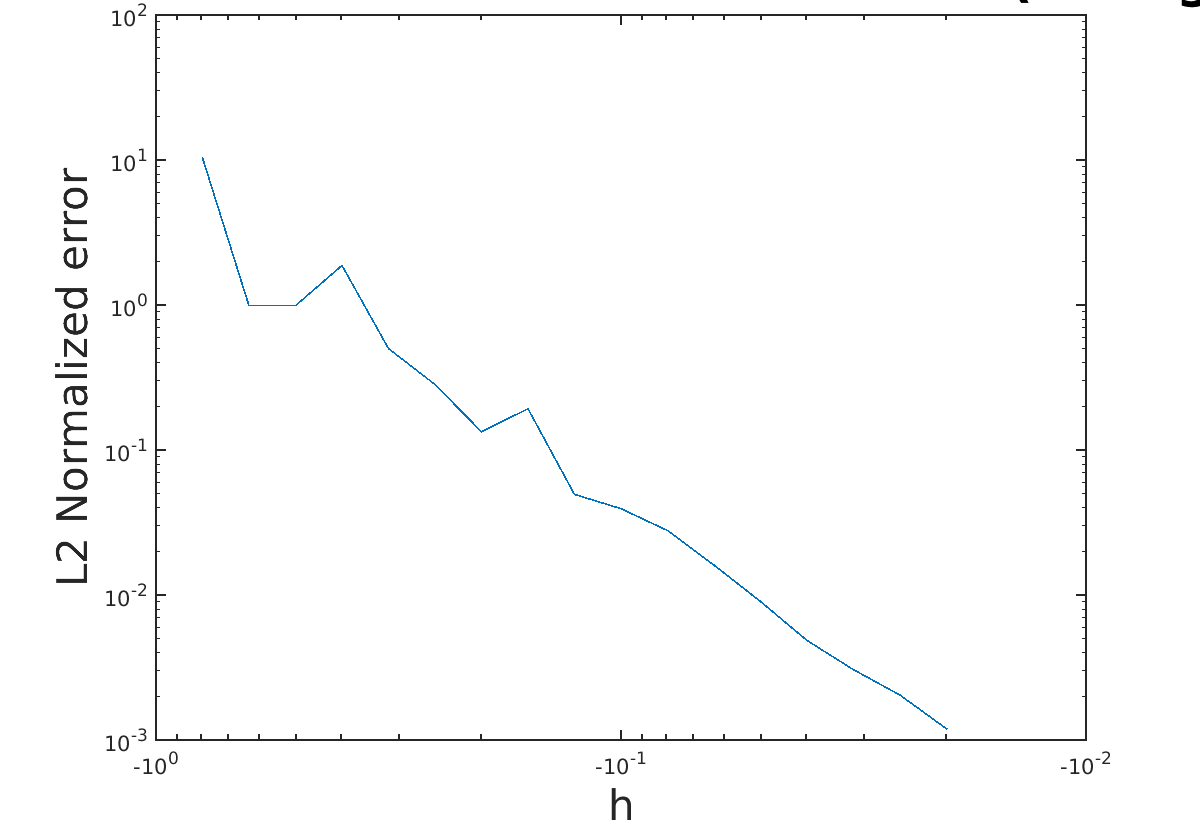
\includegraphics[width=.6\textwidth]{L2_Acst} \\
  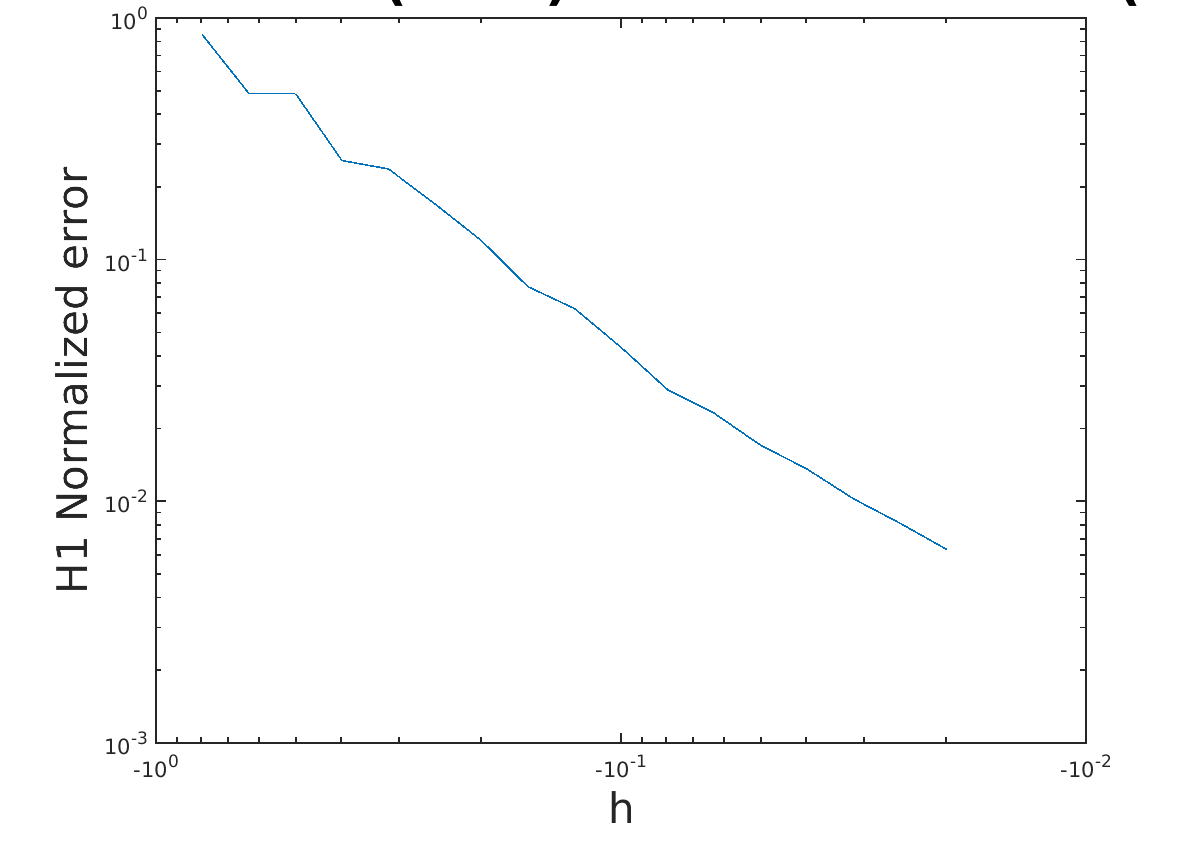
\includegraphics[width=.6\textwidth]{H1_Acst}
  \caption{Erreur normalisée pour la norme L2 et erreur normalisée pour la norme H1 dans le cas A constant.}
  \label{fig:acst}
\end{figure}


\section{Q13-16}

Cf codes commenté dans \texttt{matK\_elem.m} et \autoref{fig:avar}. Pour ce qui du calcul de la fonction $f(x,y)$, grace au code python de calcul formel, on peut trouver que pour
\begin{equation}
  A(x,y)=(\sin(\alpha \pi x)\sin(\alpha \pi y) + 2)
\end{equation}
et si on veut garder comme solution
\begin{equation}
  u(x,y)=\cos(\pi x)\cos(2\pi y)
\end{equation}
il faut poser
\begin{equation}
  \begin{aligned}[t]
    f(x,y)=&~\pi^2\alpha\sin(\pi x)\sin(\pi\alpha y)\cos(2\pi y)\cos(\pi\alpha x)\\
    &- 2\pi^2\alpha\sin(2\pi y)\sin(\pi\alpha x)\cos(\pi x)\cos(\pi\alpha y) \\
    &+ 5\pi^2(\sin(\pi\alpha x)\sin(\pi\alpha y) + 2)\cos(\pi x)\cos(2\pi y) \\
    &+ \cos(\pi x)\cos(2\pi y)
  \end{aligned}
\end{equation}

\begin{figure}
  \centering
  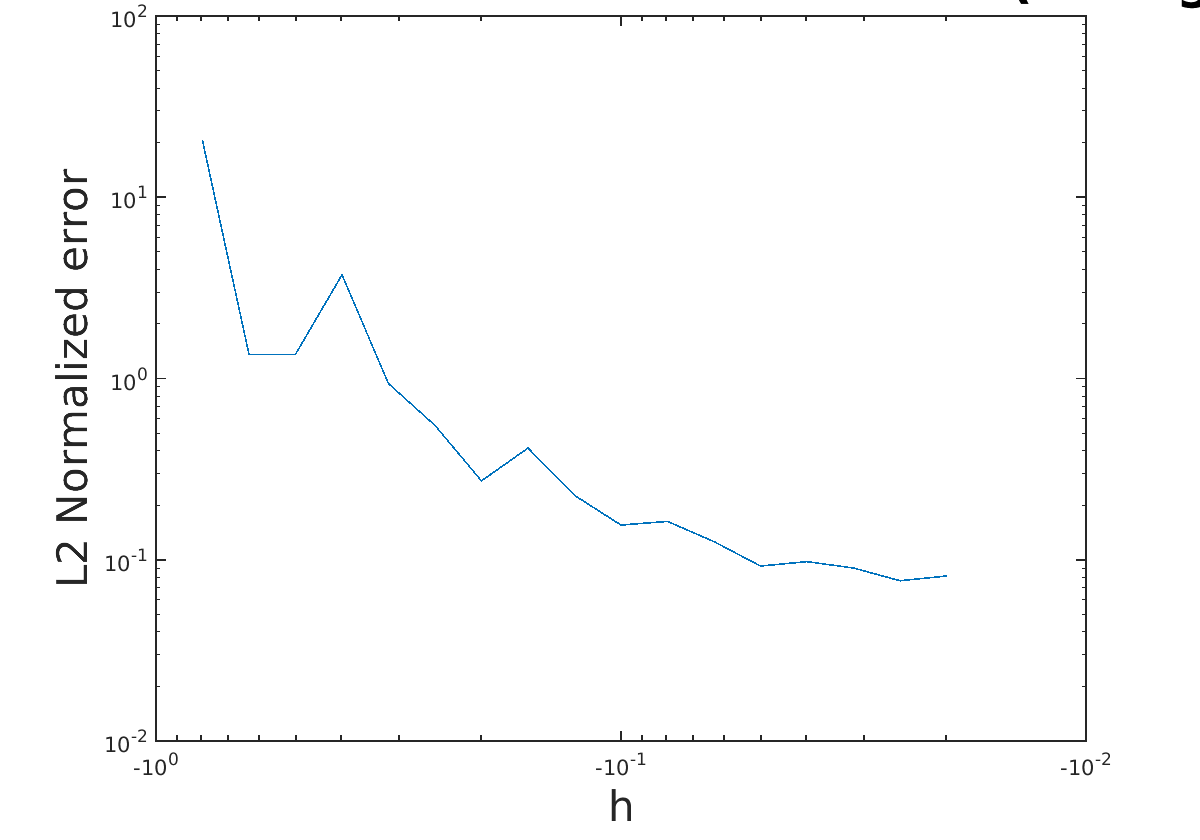
\includegraphics[width=.6\textwidth]{L2_Avar} \\
  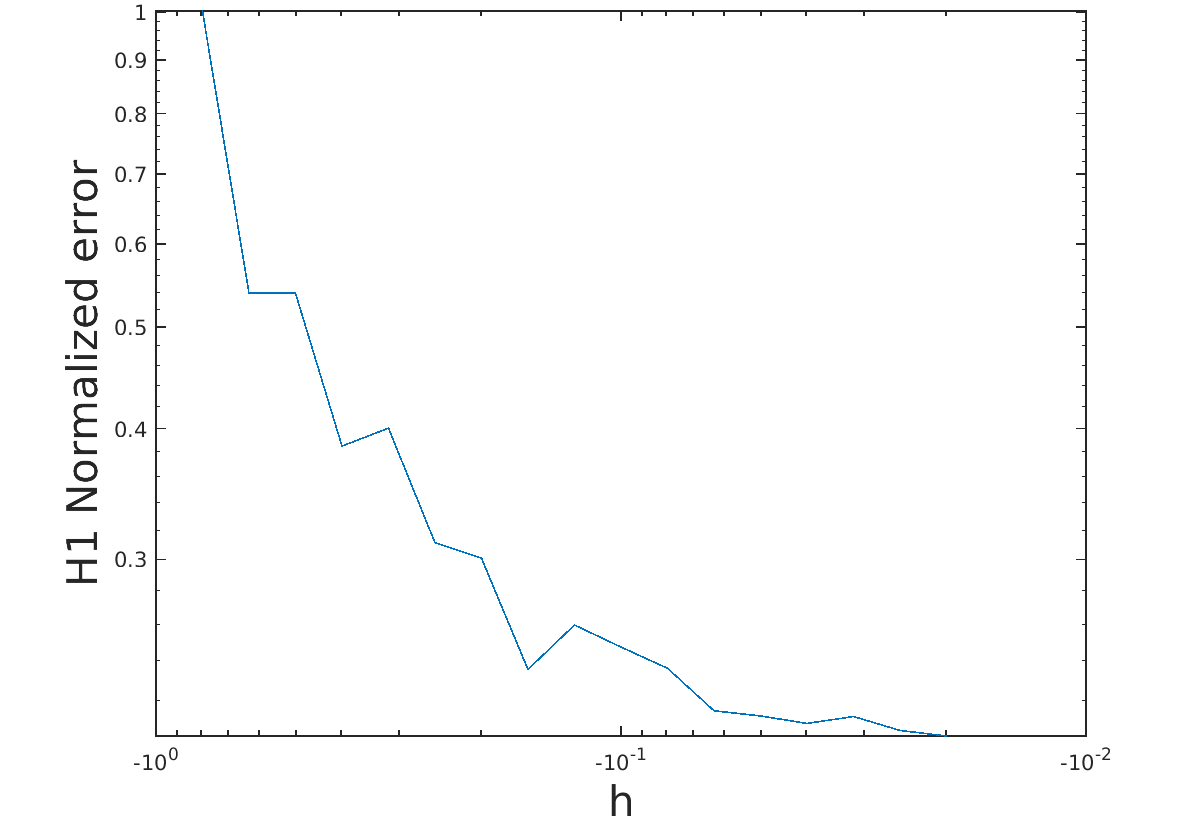
\includegraphics[width=.6\textwidth]{H1_Avar}
  \caption{Erreur normalisée pour la norme L2 et erreur normalisée pour la norme H1 dans le cas A variable.}
  \label{fig:avar}
\end{figure}

\section{Q17}

On remarque que plus $\alpha$ est grand, plus les solutions sont sensibles au pas $h$, ce qui est cohérent avec les conditions d'échantillonement des fonctions périodiques.
\end{document}

%%% Local Variables:
%%% mode: latex
%%% TeX-master: t
%%% End:
